\documentclass[a4paper,12pt,twoside]{memoir}

% Castellano
\usepackage[spanish,es-tabla]{babel}
\selectlanguage{spanish}
\usepackage[utf8]{inputenc}
\usepackage[T1]{fontenc}
\usepackage{lmodern} % Scalable font
\usepackage{microtype}
\usepackage{placeins}

\RequirePackage{booktabs}
\RequirePackage[table]{xcolor}
\RequirePackage{xtab}
\RequirePackage{multirow}

% Links
\usepackage[colorlinks]{hyperref}
\hypersetup{
	allcolors = {red}
}

% Ecuaciones
\usepackage{amsmath}

% Rutas de fichero / paquete
\newcommand{\ruta}[1]{{\sffamily #1}}

% Párrafos
\nonzeroparskip


% Imagenes
\usepackage{graphicx}
\newcommand{\imagen}[2]{
	\begin{figure}[!h]
		\centering
		\includegraphics[width=0.9\textwidth]{#1}
		\caption{#2}\label{fig:#1}
	\end{figure}
	\FloatBarrier
}

\newcommand{\imagenflotante}[2]{
	\begin{figure}%[!h]
		\centering
		\includegraphics[width=0.9\textwidth]{#1}
		\caption{#2}\label{fig:#1}
	\end{figure}
}



% El comando \figura nos permite insertar figuras comodamente, y utilizando
% siempre el mismo formato. Los parametros son:
% 1 -> Porcentaje del ancho de página que ocupará la figura (de 0 a 1)
% 2 --> Fichero de la imagen
% 3 --> Texto a pie de imagen
% 4 --> Etiqueta (label) para referencias
% 5 --> Opciones que queramos pasarle al \includegraphics
% 6 --> Opciones de posicionamiento a pasarle a \begin{figure}
\newcommand{\figuraConPosicion}[6]{%
  \setlength{\anchoFloat}{#1\textwidth}%
  \addtolength{\anchoFloat}{-4\fboxsep}%
  \setlength{\anchoFigura}{\anchoFloat}%
  \begin{figure}[#6]
    \begin{center}%
      \Ovalbox{%
        \begin{minipage}{\anchoFloat}%
          \begin{center}%
            \includegraphics[width=\anchoFigura,#5]{#2}%
            \caption{#3}%
            \label{#4}%
          \end{center}%
        \end{minipage}
      }%
    \end{center}%
  \end{figure}%
}

%
% Comando para incluir imágenes en formato apaisado (sin marco).
\newcommand{\figuraApaisadaSinMarco}[5]{%
  \begin{figure}%
    \begin{center}%
    \includegraphics[angle=90,height=#1\textheight,#5]{#2}%
    \caption{#3}%
    \label{#4}%
    \end{center}%
  \end{figure}%
}
% Para las tablas
\newcommand{\otoprule}{\midrule [\heavyrulewidth]}
%
% Nuevo comando para tablas pequeñas (menos de una página).
\newcommand{\tablaSmall}[5]{%
 \begin{table}
  \begin{center}
   \rowcolors {2}{gray!35}{}
   \begin{tabular}{#2}
    \toprule
    #4
    \otoprule
    #5
    \bottomrule
   \end{tabular}
   \caption{#1}
   \label{tabla:#3}
  \end{center}
 \end{table}
}

%
% Nuevo comando para tablas pequeñas (menos de una página).
\newcommand{\tablaSmallSinColores}[5]{%
 \begin{table}[H]
  \begin{center}
   \begin{tabular}{#2}
    \toprule
    #4
    \otoprule
    #5
    \bottomrule
   \end{tabular}
   \caption{#1}
   \label{tabla:#3}
  \end{center}
 \end{table}
}

\newcommand{\tablaApaisadaSmall}[5]{%
\begin{landscape}
  \begin{table}
   \begin{center}
    \rowcolors {2}{gray!35}{}
    \begin{tabular}{#2}
     \toprule
     #4
     \otoprule
     #5
     \bottomrule
    \end{tabular}
    \caption{#1}
    \label{tabla:#3}
   \end{center}
  \end{table}
\end{landscape}
}

%
% Nuevo comando para tablas grandes con cabecera y filas alternas coloreadas en gris.
\newcommand{\tabla}[6]{%
  \begin{center}
    \tablefirsthead{
      \toprule
      #5
      \otoprule
    }
    \tablehead{
      \multicolumn{#3}{l}{\small\sl continúa desde la página anterior}\\
      \toprule
      #5
      \otoprule
    }
    \tabletail{
      \hline
      \multicolumn{#3}{r}{\small\sl continúa en la página siguiente}\\
    }
    \tablelasttail{
      \hline
    }
    \bottomcaption{#1}
    \rowcolors {2}{gray!35}{}
    \begin{xtabular}{#2}
      #6
      \bottomrule
    \end{xtabular}
    \label{tabla:#4}
  \end{center}
}

%
% Nuevo comando para tablas grandes con cabecera.
\newcommand{\tablaSinColores}[6]{%
  \begin{center}
    \tablefirsthead{
      \toprule
      #5
      \otoprule
    }
    \tablehead{
      \multicolumn{#3}{l}{\small\sl continúa desde la página anterior}\\
      \toprule
      #5
      \otoprule
    }
    \tabletail{
      \hline
      \multicolumn{#3}{r}{\small\sl continúa en la página siguiente}\\
    }
    \tablelasttail{
      \hline
    }
    \bottomcaption{#1}
    \begin{xtabular}{#2}
      #6
      \bottomrule
    \end{xtabular}
    \label{tabla:#4}
  \end{center}
}

%
% Nuevo comando para tablas grandes sin cabecera.
\newcommand{\tablaSinCabecera}[5]{%
  \begin{center}
    \tablefirsthead{
      \toprule
    }
    \tablehead{
      \multicolumn{#3}{l}{\small\sl continúa desde la página anterior}\\
      \hline
    }
    \tabletail{
      \hline
      \multicolumn{#3}{r}{\small\sl continúa en la página siguiente}\\
    }
    \tablelasttail{
      \hline
    }
    \bottomcaption{#1}
  \begin{xtabular}{#2}
    #5
   \bottomrule
  \end{xtabular}
  \label{tabla:#4}
  \end{center}
}



\definecolor{cgoLight}{HTML}{EEEEEE}
\definecolor{cgoExtralight}{HTML}{FFFFFF}

%
% Nuevo comando para tablas grandes sin cabecera.
\newcommand{\tablaSinCabeceraConBandas}[5]{%
  \begin{center}
    \tablefirsthead{
      \toprule
    }
    \tablehead{
      \multicolumn{#3}{l}{\small\sl continúa desde la página anterior}\\
      \hline
    }
    \tabletail{
      \hline
      \multicolumn{#3}{r}{\small\sl continúa en la página siguiente}\\
    }
    \tablelasttail{
      \hline
    }
    \bottomcaption{#1}
    \rowcolors[]{1}{cgoExtralight}{cgoLight}

  \begin{xtabular}{#2}
    #5
   \bottomrule
  \end{xtabular}
  \label{tabla:#4}
  \end{center}
}


















\graphicspath{ {./img/} }

% Capítulos
\chapterstyle{bianchi}
\newcommand{\capitulo}[2]{
	\setcounter{chapter}{#1}
	\setcounter{section}{0}
	\chapter*{#2}
	\addcontentsline{toc}{chapter}{#2}
	\markboth{#2}{#2}
}

% Apéndices
\renewcommand{\appendixname}{Apéndice}
\renewcommand*\cftappendixname{\appendixname}

\newcommand{\apendice}[1]{
	%\renewcommand{\thechapter}{A}
	\chapter{#1}
}

\renewcommand*\cftappendixname{\appendixname\ }

% Formato de portada
\makeatletter
\usepackage{xcolor}
\newcommand{\tutor}[1]{\def\@tutor{#1}}
\newcommand{\course}[1]{\def\@course{#1}}
\definecolor{cpardoBox}{HTML}{E6E6FF}
\def\maketitle{
  \null
  \thispagestyle{empty}
  % Cabecera ----------------
\noindent
\includegraphics[width=\textwidth]{cabecera}\vspace{1cm}%
  \vfill
  % Título proyecto y escudo informática ----------------
  \colorbox{cpardoBox}{%
    \begin{minipage}{.8\textwidth}
      \vspace{.5cm}\Large
      \begin{center}
      \textbf{TFG del Grado en Ingeniería Informática}\vspace{.6cm}\\
      \textbf{\LARGE\@title{}}
      \end{center}
      \vspace{.2cm}
    \end{minipage}

  }%
  \hfill\begin{minipage}{.20\textwidth}
    
\includegraphics[width=\textwidth]{escudoInfor}
  \end{minipage}
  \vfill
  % Datos de alumno, curso y tutores ------------------
  \begin{center}%
  {%
    \noindent\LARGE
    Presentado por \@author{}\\ 
    en Universidad de Burgos --- \@date{}\\
    Tutor: \@tutor{}\\
  }%
  \end{center}%
  \null
  \cleardoublepage
  }
\makeatother

\newcommand{\nombre}{Nombre del alumno} %%% cambio de comando

% Datos de portada
\title{título del TFG}
\author{\nombre}
\tutor{nombre tutor}
\date{\today}

\begin{document}

\maketitle


\newpage\null\thispagestyle{empty}\newpage


%%%%%%%%%%%%%%%%%%%%%%%%%%%%%%%%%%%%%%%%%%%%%%%%%%%%%%%%%%%%%%%%%%%%%%%%%%%%%%%%%%%%%%%%
\thispagestyle{empty}


\noindent
\includegraphics[width=\textwidth]{cabecera}\vspace{1cm}

\noindent D. nombre tutor, profesor del departamento de nombre departamento, área de nombre área.

\noindent Expone:

\noindent Que el alumno D. \nombre, con DNI dni, ha realizado el Trabajo final de Grado en Ingeniería Informática titulado título de TFG. 

\noindent Y que dicho trabajo ha sido realizado por el alumno bajo la dirección del que suscribe, en virtud de lo cual se autoriza su presentación y defensa.

\begin{center} %\large
En Burgos, {\large \today}
\end{center}

\vfill\vfill\vfill

% Author and supervisor
\begin{minipage}{0.45\textwidth}
\begin{flushleft} %\large
Vº. Bº. del Tutor:\\[2cm]
D. nombre tutor
\end{flushleft}
\end{minipage}
\hfill
\begin{minipage}{0.45\textwidth}
\begin{flushleft} %\large
Vº. Bº. del co-tutor:\\[2cm]
D. nombre co-tutor
\end{flushleft}
\end{minipage}
\hfill

\vfill

% para casos con solo un tutor comentar lo anterior
% y descomentar lo siguiente
%Vº. Bº. del Tutor:\\[2cm]
%D. nombre tutor


\newpage\null\thispagestyle{empty}\newpage




\frontmatter

% Abstract en castellano
\renewcommand*\abstractname{Resumen}
\begin{abstract}
En este primer apartado se hace una \textbf{breve} presentación del tema que se aborda en el proyecto.
\end{abstract}

\renewcommand*\abstractname{Descriptores}
\begin{abstract}
Palabras separadas por comas que identifiquen el contenido del proyecto Ej: servidor web, buscador de vuelos, android \ldots
\end{abstract}

\clearpage

% Abstract en inglés
\renewcommand*\abstractname{Abstract}
\begin{abstract}
A \textbf{brief} presentation of the topic addressed in the project.
\end{abstract}

\renewcommand*\abstractname{Keywords}
\begin{abstract}
keywords separated by commas.
\end{abstract}

\clearpage

% Indices
\tableofcontents

\clearpage

\listoffigures

\clearpage

\listoftables
\clearpage

\mainmatter
\capitulo{1}{Introducción}

Descripción del contenido del trabajo y del estrucutra de la memoria y del resto de materiales entregados.

\capitulo{2}{Objetivos del proyecto}

Este apartado explica de forma precisa y concisa cuales son los objetivos que se persiguen con la realización del proyecto. Se puede distinguir entre los objetivos marcados por los requisitos del software a construir y los objetivos de carácter técnico que plantea a la hora de llevar a la práctica el proyecto.

En esta sección se listan los objetivos que persigue la realización del proyecto, tanto 

\subsection{Objetivos principales}
\begin{itemize}
	\tightlist
	\item Desarrollar una aplicación que proporcione las opciones de procesamiento más comunes.
	\item Que la aplicación final sea útil para la investigadora.
	\item La aplicación tiene que ser usable e intuitiva.
	\item Que la herramienta se consiga desplegar.
	\item Ofrecer control de usuarios para que cada uno pueda almacenar sus archivos.
	\item Ofrecer un sistema de aprendizaje automático para ayudar en la clasificación de futuras muestras de espectros.
\end{itemize}

\subsection{Objetivos técnicos}
\begin{itemize}
	\tightlist
	\item Que la aplicación sea fácil de mantener.
	\item Utilizar git como sistema de control de versiones junto con GitHub para el repositorio remoto.
	\item Utilizar una metodología ágil, Scrum, para el desarrollo.
	\item Utilizar un sistema kanban para la gestión de tareas.
	\item Utilizar un sistema de revisión automática de código para asegurar su calidad.
	\item Utilizar un sistema de integración continua.
\end{itemize}

\subsection{Objetivos personales}
\begin{itemize}
	\tightlist
	\item Ampliar los conocimientos sobre desarrollo web a partir de los obtenidos durante el grado.
	\item Ampliar y profundizar conocimientos sobre Python, especialmente en desarrollo web y aprendizaje automático.
	\item Aprender a usar técnicas de aprendizaje automático en un entorno de investigación real.
	\item Desarrollar el proyecto de la forma más profesional posible.
\end{itemize}
\capitulo{3}{Conceptos teóricos}

En aquellos proyectos que necesiten para su comprensión y desarrollo de unos
conceptos teóricos de una determinada materia o de un determinado dominio de
conocimiento, debe existir un apartado que sintetice dichos conceptos.

Algunos conceptos teóricos de \LaTeX \footnote{Créditos a los proyectos de
	Álvaro López Cantero: Configurador de Presupuestos y Roberto Izquierdo Amo:
	PLQuiz}.

\section{Secciones}

Las secciones se incluyen con el comando section.

\subsection{Subsecciones}

Además de secciones tenemos subsecciones.

\subsubsection{Subsubsecciones}

Y subsecciones. 


\section{Referencias}

Las referencias se incluyen en el texto usando cite \cite{wiki:latex}. Para
citar webs, artículos o libros \cite{koza92}.


\section{Imágenes}

Se pueden incluir imágenes con los comandos standard de \LaTeX, pero esta
plantilla dispone de comandos propios como por ejemplo el siguiente:

\imagen{escudoInfor}{Autómata para una expresión vacía}



\section{Listas de items}

Existen tres posibilidades:

\begin{itemize}
	\item primer item.
	\item segundo item.
\end{itemize}

\begin{enumerate}
	\item primer item.
	\item segundo item.
\end{enumerate}

\begin{description}
	\item[Primer item] más información sobre el primer item.
	\item[Segundo item] más información sobre el segundo item.
\end{description}

\begin{itemize}
	\item 
\end{itemize}

\section{Tablas}

Igualmente se pueden usar los comandos específicos de \LaTeX o bien usar alguno
de los comandos de la plantilla.

\tablaSmall{Herramientas y tecnologías utilizadas en cada parte del proyecto}{l
	c c c c}{herramientasportipodeuso}
{ \multicolumn{1}{l}{Herramientas} & App AngularJS & API REST & BD & Memoria
	\\}{ 
	HTML5 & X & & &\\
	CSS3 & X & & &\\
	BOOTSTRAP & X & & &\\
	JavaScript & X & & &\\
	AngularJS & X & & &\\
	Bower & X & & &\\
	PHP & & X & &\\
	Karma + Jasmine & X & & &\\
	Slim framework & & X & &\\
	Idiorm & & X & &\\
	Composer & & X & &\\
	JSON & X & X & &\\
	PhpStorm & X & X & &\\
	MySQL & & & X &\\
	PhpMyAdmin & & & X &\\
	Git + BitBucket & X & X & X & X\\
	Mik\TeX{} & & & & X\\
	\TeX{}Maker & & & & X\\
	Astah & & & & X\\
	Balsamiq Mockups & X & & &\\
	VersionOne & X & X & X & X\\
} 


\capitulo{4}{Técnicas y herramientas}

\section{Librerías de representación}

\subsection{Dash}
Librería en Python que permite crear sitios webs completos para representación de datos. Para ello hace uso de diversas tecnologías, \textit{Flask} para el servidor web, \textit{Plotly} para la representación y \textit{React} para los componentes y actualización.
\subsubsection{Pros}
\begin{itemize}
	\item Gráficos interactivos
	\item Fácil actualización del gráfico en la web mediante \verb|@app.callback|
	\item Integración de elementos HTML para la actualización del gráfico
	\item Uso de la librería \textit{cufflinks} para unir generar una figura directamente de un \textit{DataFrame}
	\item Al ser de los creadores de \textit{Plotly} y usarlo internamente da la posibilidad de usar sus componentes
	\item Al usar \textit{Flask} como servidor tiene acceso a todas sus ventajas
\end{itemize}
\subsubsection{Contras}
\begin{itemize}
	\item El código HTML hay que escribirlo desde el código de Python, esto hace que se complique el mantenimiento
	\item No se pueden reutilizar las plantillas de \textit{Flask}
\end{itemize}

\subsection{Plotly}
Plataforma para representación de datos, dispone de varias librerías para diferentes lenguajes de programación. Representación online y offline.
\subsubsection{Pros}
\begin{itemize}
	\item Gráficos interactivos
	\item Posibilidad de uso con \textit{Flask} y \textit{Jupyter}
\end{itemize}
\subsubsection{Contras}
\begin{itemize}
	\item Para representar en la web hay que hacer uso de dos versiones de la librería, para Python y para JavaScript
	\item La representación online guarda los gráficos generados en una cuenta asociada de la plataforma
	\item La representación offline devuelve el gráfico en Python, pero para representarlo es necesario convertirlo a JSON, enviarlo a la web y que la parte de JS lo represente
	\item La actualización es necesaria hacerla desde el cliente con JS, donde no se dispone de los datos ni de las utilidades de minería de datos
\end{itemize}

\section{Infraestructura}
\subsection{Jupyter Notebook}
Aplicación web que permite la edición y ejecución de código, Python en este caso, en el navegador, donde también se muestran el resultado de la ejecución. Dispone de \textit{widgets} para interactuar con el programa. Se instala localmente.
\subsubsection{Pros}
\begin{itemize}
	\item Fácil subir archivos al servidor en el menú principal
	\item Al no tener que hacer una interfaz web permite centrarse en la programación del código de minería de datos
	\item Los gráficos generados con \textit{Plotly} se representan directamente en el notebook
	\item Posibilidad de usar \url{https://mybinder.org/} para el despliegue
	\item Actualización del gráfico por medio de los \textit{widgets} e \verb|interact|
\end{itemize}
\subsubsection{Contras}
\begin{itemize}
	\item Menos usable e intuitivo
	\item Al estar el código expuesto el cliente podría alterarlo sin querer
	\item \href{http://jupyter-notebook.readthedocs.io/en/latest/public_server.html}{Solo se puede un usuario en servidor público}
\end{itemize}

\subsection{Flask}
Microframework para aplicaciones web en Python. Aunque por si solo \textit{Flask} no sea muy completo, dispone de una gran cantidad de extensiones oficiales y de la comunidad para suplir todas las características de un framework web completo.
\subsubsection{Pros}
\begin{itemize}
	\item Maneja bien la subida de ficheros
	\item Al ser web hay más control sobre lo que puede hacer el usuario y sobre lo que se le presenta, con la finalidad de hacer más usable la aplicación
	\item Reutilización de código HTML mediante plantillas y macros
\end{itemize}
\subsubsection{Contras}
\begin{itemize}
	\item Mucho más trabajo al tener que diseñar y programar la interfaz web
\end{itemize}

\section{Despliegue}
\url{https://www.youtube.com/watch?v=vGphzPLemZE}\\
\url{https://gumroad.com/l/python-deployments}\\
\url{https://www.fullstackpython.com/platform-as-a-service.html}\\
\url{https://www.fullstackpython.com/servers.html}
\subsection{Heroku}
Plataforma como servicio, la forma más fácil de despliegue. Tan escalable como fondo tenga la cartera. \url{https://www.heroku.com/}\\

El almacenamiento no es permanente, hay que usar servicios de terceros y conectarlos mediante plugin.
\subsection{Ngrok}
Túnel seguro desde Internet hasta un servidor local en tu máquina. Dirección aleatoria cada vez que se enciende. \url{https://ngrok.com/}\\

El almacenamiento es permanente porque es el almacenamiento de la máquina.
\subsection{Digital Ocean}
Solo de pago pero de momento está disponible por el pack educacional de GitHub. Tan escalable como fondo tenga la cartera. VPS.\\ \url{https://www.digitalocean.com/}\\ \url{https://pythonprogramming.net/basic-flask-website-tutorial/}\\

Dispone del almacenamiento que ofrece la máquina virtual, es permanente. En caso de que ese espacio sea insuficiente se puede agregar más pagando.
\subsection{Google App Engine, Google Cloud Platform}
Despliegue de Google como plataforma como servicio o VPS. Periodo de prueba gratis y luego tan escalable como fondo tenga la cartera. Funciona con Python 2.7\\
\url{https://cloud.google.com/appengine/docs/standard/python/getting-started/python-standard-env}\\
\url{https://cloud.google.com/appengine/docs/standard/python/tools/uploadinganapp}\\
\url{https://cloud.google.com/python/getting-started/hello-world}\\
\url{https://cloud.google.com/appengine/docs/flexible/python/quickstart}\\

Ofrece formas de almacenamiento de Google como Cloud Storage para ficheros, caso que nos interesa, hay que pagar por ellas.
\subsection{Open Shitf}
Plataforma como servicio. Plan básico gratis y plan profesional de pago, tan escalable como fondo tenga la cartera.\\
\url{https://www.openshift.com/}\\
\url{https://blog.openshift.com/beginners-guide-to-writing-flask-apps-on-openshift/}\\
\url{https://blog.openshift.com/how-to-install-and-configure-a-python-flask-dev-environment-deploy-to-openshift/}\\

No ofrece almacenamiento por defecto, lo ofrece por medio de lo que llaman ``PersistentVolume'', ofrecen una API para comunicarse con ello.
\subsection{PythonAnywhere} 
Plataforma como servicio especializada en Python. Varios planes, a mejor plan más caro. El plan más básico es gratis.\\
\url{https://www.pythonanywhere.com/}\\
\url{https://www.youtube.com/watch?v=M-QRwEEZ9-8}\\
Ofrecen almacenamiento de serie pero muy limitado y de pago.
\subsection{AWS Elastic Beanstalk,  AWS CodeStar}
Solución en la nube de Amazon. VPS. Tan escalable como fondo tenga la cartera.\\
\url{https://aws.amazon.com/es/elasticbeanstalk/}\\
\url{https://aws.amazon.com/es/codestar/}\\

Al igual que en el caso de Google, ofrece almacenamiento persistente con sus servicios, Amazon S3, los cuales hay que pagar.
\subsection{AWS Lambda, Zappa}
Zappa es un capa por encima de AWS Lambda para desplegar en modo \textit{serverless}. AWS Lambda se ocupa del escalado y Zappa del despliegue.\\
\url{https://github.com/Miserlou/Zappa}\\

Solo almacenamiento temporal.
\subsection{Docker}
Despliegue en contenedores.\\
\url{https://www.docker.com/}\\

De serie no tiene almacenamiento persistente pero es capaz de ofrecerlo mediante ``storage drivers''. Requiere bastante configuración.
\subsection{Azure}
Solución en la nube de Microsoft. VPS. Tan escalable como fondo tenga la cartera.\\
\url{https://azure.microsoft.com/es-es/}\\
\url{https://docs.microsoft.com/en-us/azure/app-service/app-service-web-get-started-python}\\

Sí ofrece almacenamiento persistente.
\subsection{Nanobox}
Solución interesante, combina los contenedores de Docker con despliegue en la nube y lo automatiza. De momento compatibilidad con Digital Ocean, Amazon y Linode, Google, Joyent y Azure en camino. Plan básico gratis, el resto de precios son flexibles. También en local.\\
\url{https://nanobox.io/}\\
\url{https://github.com/nanobox-io/nanobox}\\

Ofrece almacenamiento persistente, hay que configurar las rutas que van a ser persistentes en el fichero de configuración. Cada despliegue el almacenamiento que se haya usado so borra. Depende del almacenamiento que esté disponible en el servicio escogido para almacenar.
\capitulo{5}{Aspectos relevantes del desarrollo del proyecto}

En este apartado se van a recoger los aspectos más importantes del desarrollo
del proyecto. Desde las decisiones que se tomaron y sus implicaciones,
hasta los numerosos problemas a los que hubo que enfrentarse y cómo se
solucionaron.

\section{Elección del proyecto}

A finales del curso pasado se organizó una charla en la que los profesores iban
a presentar las optativas que daban clase de forma que los alumnos tuviéramos
más fácil elegir asignaturas. En la presentación de la asignatura ``Minería de
Datos'' despertó interés por el tema y se preguntó a José Francisco, por haber
realizado la presentación, sobre TFGs relacionados con el tema.

De los trabajos disponibles este llamó la atención por estar relacionados con
geología y con desarrollo web, además de poder aplicar técnicas minería de datos
en un entorno real de investigación.

\section{Formación}

Para poder realizar el proyecto se necesitaban unos conocimientos no adquiridos
sobre desarrollo web, tanto de la parte de servidor en Flask como la parte del
cliente en HTML, CSS y JavaScript, aunque en menor medida por haberse tocado
algo durante el grado. Como se había hablado con los tutores antes de verano
sobre el proyecto, se dedicó parte a aprender sobre ello. Además de para
aprendizaje, los recursos se han usado también como material de consulta durante
el desarrollo.

\noindent Para la parte del servidor se siguieron los libros y tutoriales:
\begin{itemize}
	\item Flask Web Development~\cite{grinberg2014flask}
	\item Explore Flask~\cite{exploreflask}
	\item The Flask Mega-Tutorial Legacy (2012)~\cite{grinberg-mega-legacy}
	\item The Flask Mega-Tutorial (2017)~\cite{grinberg-mega}
\end{itemize}

\noindent Para la parte del cliente se utilizaron principalmente los siguientes
materiales:
\begin{itemize}
	\item MDN Web Docs~\cite{mdn}
	\item W3Schools Tutorials~\cite{w3schools}
\end{itemize}

A medida que se añadían nuevas herramientas al proyecto, su documentación
oficial también ha sido consultada en varias ocasiones, están disponibles en:
\begin{itemize}
	\item Documentación de Flask~\cite{doc:flask}
	\item Documentación de Bootstrap~\cite{doc:bootstrap}
	\item Documentación de Nanobox~\cite{doc:nanobox}
	\item Documentación de PyMongo~\cite{doc:pymongo}
	\item Documentación de Dash~\cite{doc:dash}
	\item Documentación de Plotly~\cite{doc:plotly}
\end{itemize}

\section{Sistema de usuarios}

Uno de los primeros problemas que se plantearon fue la forma de ofrecer el
sistema de usuarios, para que cada uno pudiera almacenar sus archivos. Las
opciones que se presentaban eran implementar uno desde cero con ayuda de las
extensiones que ofrece Flask o mediante un sistema de terceros, como puede ser
Google.

Implementar el sistema desde cero tenía la ventaja de que los usuarios no tenían
que salir de la página para iniciar sesión y que se había aprendido como hacerlo
en los tutoriales sobre Flask mencionados anteriormente, mientras que el sistema
de terceros no se sabía como hacerlo, pero tenía más ventajas, siendo las
principales no tener que mantener una base de datos de usuarios, no depender de
un sistema de envío de correo electrónico (dio problemas en proyectos
anteriores) y no tener que obligar a los usuarios a crearse otra cuenta al poder
usar una existente.

Al final se decidió usar la autenticación con Google, por estar casi garantizado
que los usuarios van a tener una cuenta existente, la documentación sobre este
aspecto es abundante y era fácil de implementar. Además al iniciar sesión con
este servicio nos permite usar la API de Google para obtener los datos del
usuario necesarios.

\section{Cohesión entre Flask y Dash}

Al contar con la presencia de dos \textit{frameworks} de desarrollo web hacer
que funcionen juntos ha sido un reto, sobre todo teniendo en cuenta que Dash se
ejecuta Flask pero no permite reutilizar sus componentes, favoreciendo la
aparición de código repetido y disminuyendo la mantenibilidad.

El mayor problema que se ha tenido ha sido la diferencia en como escribir el
código HTML para la interfaz en el cliente. Mientras que en Flask se escribe en
ficheros HTML llamados \textit{templates}, Dash apuesta por escribir todo el
código desde Python. Esto favorece que surjan defectos de código, sobre todo de
código duplicado.

Se investigó bastante sobre cómo poder usar los \textit{templates} de Flask para
definir la interfaz de Dash, pero no se pudo encontrar forma de poder hacerlo. Al
final no quedó otra forma de hacerlo, pero dentro de lo malo es un pequeño
precio a pagar por el resto de ventajas que Dash ofrece.

\section{Subida de ficheros}\label{sec:subida}

Una de las primeras características que se implementó fue la subida de ficheros
al servidor, al tener ya el sistema de usuarios, se podían organizar los datos
sin problema para cada cliente. El formato requerido para subir los datos pasó
por varios cambios motivados por la forma en la que la Dra. Jorge Villa nos
enviaba los datos que probar la aplicación. En secciones posteriores se explica
como estos cambios afectaron también al almacenamiento de los datos y la
interfaz del visor.

\subsection{Organización en directorios}\label{sec:directorios}

Al principio, los datos se encontraban organizados en directorios cuyo nombre
proporcionaba toda la información sobre los ejemplos que contenían. Por lo que
el formato que se pedía era simple, un archivo comprimido en formato \code{.zip}
que contuviera estos directorios.

\subsection{Estructura según hoja de metadatos}\label{sec:excel}

Sobre mediados de abril los nuevos datos recibidos empezaron a estar organizados
según una hoja de Excel que relacionaba los nombres de directorios y los
ejemplos que contenían con sus metadatos, en vez de estar contenidos en el
nombre.

Esta hoja contenía una columna llamada \code{Id} con el nombre de un directorio y
los ejemplos de ese tipo, las siguientes columnas contenían datos sobre los
ejemplos contenidos en esa fila, como la mina de la que han sido extraídas las
muestras o la profundidad.

Esta hoja se adaptó para aplicación manteniendo la columna \code{Id} y añadiendo
fijas una columna para la mina y otras dos para la profundidad, una nominal y
otra numérica. El formato de subida pasó a ser en un mismo fichero \code{.zip} los
directorios que contienen los ejemplos y la hoja con los metadatos previamente
cumplimentada.

\section{Interfaz del visor}

Esta parte del proyecto está muy relacionado con lo explicado en la
sección~\ref{sec:subida}, el usuario del visor espera que se le presenten los
datos de una forma similar a como los ha subido.

Cuando los datos se subían como un archivo comprimido con carpetas cuyo nombre
contiene la información, se presentaban al usuario dos menús desplegables. En la
carga, solo uno de ellos contenía valores, los nombres de los directorios. El
segundo desplegable actualizaba sus valores con los nombres de los ficheros
contenidos en la carpeta seleccionada, al seleccionar el fichero se cargaba en
el visor.

Con el cambio de la hoja con metadatos, el tutor Dr. Díez Pastor propuso que al
usuario se le mostrase una tabla parecida a la hoja que había rellenado antes de
subir los datos, con la diferencia de que se mostrasen todos los ficheros como
filas con sus metadatos, asemejándose a la estructura final de almacenamiento de
datos.

Mostrar los datos al usuario en forma de tabla trajo las ventajas de poder
representar varios espectros a la vez, filtrar y ordenar según las columnas (ver
figura~\ref{fig:tabla-espectros}).

\imagen{tabla-espectros}{Tabla de espectros} 

\section{Almacenamiento de datos}

El principal motivo de implementar un sistema de usuarios fue que cada uno
pudiera tener sus datos almacenados para no tener que subirlos cada vez que se
quiera trabajar con ellos.

\subsection{Inicialmente}

Al principio, se almacenaban directamente en un directorio nombrado como el
identificador del usuario y lo único que se hacía era descomprimir el archivo
comprimido en ese directorio. Esta forma de almacenar los datos conlleva varios
problemas que motivaron el cambio en la forma de almacenamiento a la actual.
Esta forma de almacenamiento se corresponde al formato explicado en la
sección~\ref{sec:directorios}.

El problema más evidente, y que más notarían los usuarios, es que, cada vez que
se quisiera ver un espectro, hay que cargarlo desde el disco, disminuyendo el
rendimiento general de la aplicación.

Otro gran problema de esta forma de almacenar era como manejaba el servidor los
ficheros guardados, este tema se explicará más en detalle en la
sección~\ref{sec:despliegue}.

El último problema, y el más problemático desde el punto de vista de programación,
es que para cada operación que se quisiera realizar con los datos se necesitaban
escribir funciones auxiliares complejas para buscar y manipular el árbol de
directorios, las cuáles había que modificar con cada cambio en la estructura,
dificultando el mantenimiento de la aplicación.

Se planteó cambiar la forma de almacenar los datos en el servidor, cambio que
terminó por realizarse después de valorar ventajas y desventajas en este momento
del desarrollo.

\subsection{Migración a MongoDB}\label{sec:migrate-mongo}

Por sugerencia del tutor se investigó la posibilidad de usar MongoDB para
almacenar los datos. Se vio que podría funcionar realmente bien al poder
insertar directamente los ficheros cargados en la base de datos, recuperarlos y
borrarlos fácilmente. Como consecuencia directa del cambio, los métodos
auxiliares con los que se interactuaba con los datos disminuyeron
considerablemente en tamaño y complejidad.

En primera instancia se optó por guardar los conjuntos de datos como un
documento en el que estaban contenidos varios \textit{DataFrames} (cada uno
representando un espectro) agrupados según la carpeta en la que estuvieran
localizados los espectros. Cada \textit{DataFrame} contenía dos columnas, una
con los valores del eje X y otra con los valores del eje Y.

Pero justo a continuación de adoptar esta estructura y tener la aplicación
adaptada para ello llegó el cambio en como recibíamos los datos, provocando otra
modificación en la estructura. Esta vez se decidió agrupar todo el conjunto de
datos subido en un solo \textit{DataFrame}, en el que cada fila se corresponde
con un espectro, las columnas representan el eje X y los valores de cada fila en
esas columnas representan el valor del eje Y. Cada fila contiene adicionalmente
columnas que indican el nombre del espectro y sus metadatos asociados (ver
figura~\ref{fig:dataframe-def}). En la sección~\ref{sec:integracion} se explican
más en profundidad este cambio.

\begin{figure}[!h]
	\centering
	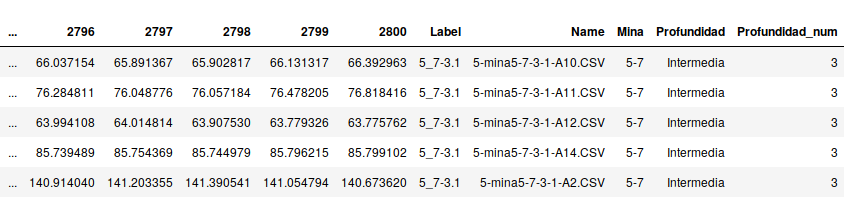
\includegraphics[width=\textwidth]{dataframe-def}
	\caption{Estructura definitiva}\label{fig:dataframe-def}
\end{figure}

Guardar los datos de esta forma facilita aplicar los métodos de minería de datos,
al estar pensado para aplicarse en lote.


\section{Integración de los algoritmos existentes}\label{sec:integracion}

Como se ha comentado en la introducción (página~\pageref{ch:introduccion}), este
proyecto surge de una colaboración. De aquí se obtuvieron bastantes algoritmos,
gran parte de ellos dedicados al procesamiento de los espectros, que se
añadieron sobre la librería ``superman''~(\ref{lib:superman}).

Una de las partes más importantes del proyecto era conseguir integrar estos
algoritmos en la aplicación web para poder ejecutarlos sobre los espectros
visualizados.

Cuando llegó el momento de integrar los algoritmos en la aplicación había dos
opciones para hacerlo funcionar, modificar la aplicación para adaptarse a los
algoritmos o modificar los algoritmos para adaptarse a la aplicación.

En primera instancia se intento modificar los algoritmos, pero se vio que era un
paquete con demasiadas dependencias dentro del mismo, por lo que cada cambio 
producía gran cantidad de errores de funcionamiento, que al solucionar 
producían todavía más errores dentro del paquete. Se optó por revertir estos
cambios y modificar la aplicación.

La modificación principal fue el último cambio comentado en la 
sección~\ref{sec:migrate-mongo} (figura~\ref{fig:dataframe-def}). Con esa 
modificación el funcionamiento de la aplicación volvió a ser el correcto.

\section{Despliegue}\label{sec:despliegue}

La idea de realizar el proyecto como una aplicación web tiene relación más que
directa con que pueda ser fácilmente accesible. Para ello se necesita que
esté desplegada y accesible en Internet. En esta sección de describe las etapas
por las que pasó el despliegue, los problemas que surgieron y cómo se
solucionaron.

En las primeras reuniones del proyecto se comentó, con los tutores que un gran
problema de los proyectos anteriores desarrollados en web se centraban en el
despliegue al final del proyecto, haciendo que alguna vez no pudieran llegarse a
desplegar, por eso se planteó la idea de empezar a desplegar desde el inicio del
proyecto.

\subsection{Servidor}

La plataforma escogida fue \hrefFootnote{https://www.heroku.com/}{Heroku}
por su simplicidad y un plan gratuito que cubre las necesidades del proyecto.
Aunque en primera instancia parecía que esta plataforma funcionaba bien para
nuestras necesidades, se vio que no contaba con almacenamiento persistente,
convirtiendo su uso en inviable.

Las opciones que se plantearon fueron buscar una forma de añadir este
almacenamiento y cambiar de servidor por completo. Para añadirlo en Heroku había
que depender de complementos externos para enlazar a servicios de 
almacenamiento de terceros teniendo que modificar la aplicación para hacerlo
funcionar, además de ser servicios de pago.

Al final se escogió por cambiar a un proveedor \textit{cloud} de pago que
ofreciese máquinas virtuales privadas, las opciones manejadas fueron
\hrefFootnote{https://www.digitalocean.com/}{DigitalOcean},
\hrefFootnote{https://aws.amazon.com/es/}{Amazon Web Services} y
\hrefFootnote{https://cloud.google.com/}{Google Cloud}. Se escogió la primera
opción ya que gracias al
\hrefFootnote{https://education.github.com/pack}{Student Developer Pack} se
disponía de un cupón de 50\$ en esta plataforma.

\subsection{Herramientas para el despliegue}

La plataforma Heroku posee sus propias herramientas para el despliegue,
facilitando en gran cantidad este proceso. Esta plataforma usa un repositorio
\textit{git} remoto para almacenar la aplicación por lo que al contar ya con
este sistema de control de versiones en el proyecto no hubo que modificar casi
nada para poder desplegar, pero por los problemas comentados anteriormente se
tuvo que abandonar.

Para complementar a DigitalOcean y facilitar la tarea del despliegue se ha usado
el servicio \hrefFootnote{https://nanobox.io/}{Nanobox}. Al principio de usar
esta plataforma, se vio que los datos almacenados se eliminaban en cada
despliegue, para ello hubo que añadir un segundo contenedor que se ocupara del
almacenamiento, lo bueno es que este contenedor se asocia a un directorio del
servidor, por lo que la aplicación no se tuvo que modificar. Más adelante se
añadió otro contenedor para gestionar la base de datos MongoDB.

\section{Creación de clasificadores}

Dentro del objetivo de aplicación de técnicas de minería de datos había que
decidir si dejar a los usuarios la opción de crear clasificadores personalizados
o simplemente entrenarlos a partir de \textit{datasets} subidos. Se decidió
probar la primera opción, teniendo la segunda como respaldo en caso de no
funcionar.

\subsection{Obtención de parámetros}

Para conseguir esta personalización surge el problema de cómo obtener los
parámetros del clasificador y presentárselos al usuario. La primera idea que
surgió es analizar la documentación oficial de los clasificadores y crear a mano
un fichero con los parámetros, esto puede resultar viable si se usan pocos
clasificadores, pero dificulta mucho la adición de nuevos.

Se descartó a favor de buscar una herramienta que pudiera analizar la
documentación \textit{in-code} de los clasificadores. Al ser un formato
estructurado, y conociendo herramientas en otros lenguajes de análisis de este
tipo de documentación, se tenía la confianza de que para Python existirían
herramientas parecidas.

Efectivamente, encontró la librería \hrefFootnote{https://github.com/numpy/numpydoc}{numpydoc}
que, entre otras características, ofrece la funcionalidad que se busca, analiza
la documentación y devuelve un diccionario con las secciones, entre ellas los
parámetros.

Con esta información se puede generar un formulario automáticamente y hacer que
cambie dinámicamente según la opción del usuario.

\subsection{Procesamiento del formulario}

El servidor recibe todos los datos como si fueran cadenas, aunque el control en
el formulario sea de tipo numérico, por lo toca convertir las cadenas al tipo
correcto con un método de prueba y error, para luego guardarlos y pasárselos al
constructor del clasificador. Si no se ha introducido valor, no se guarda,
permitiendo usar el valor por defecto.

Primero, si el valor coincide con un \textit{booleano}, se convierte, si no, se
prueba a convertir en entero, si salta excepción, se prueba a convertir en
numérico con decimales, en caso de que salte excepción, al no haber más tipos
primitivos, se asume que el valor tiene que ser una cadena y guarda como tal.

\subsection{Mantener el modelo entre peticiones}

Al ser los clasificadores creados y personalizados desde la web, estos
necesariamente se tienen que crear mientras se procesa la petición, con su
consecuente destrucción al terminar de procesarla, con lo que la tarea de
guardarlos se complica.

Las ideas propuestas para solventar el problema fueron guardar los parámetros
usados como una \textit{cookie} para poder entrenar el modelo otra vez antes de
guardarlo, o serializar el modelo ya entrenado en el servidor temporalmente y
cargarlo en caso de querer guardarlo definitivamente.

A pesar de la facilidad de usar \textit{cookies} para solucionar el problema,
estos datos guardados son necesarios solo en el caso de que se elija guarda el
modelo, por lo que parece algo precipitado guardarlos cuando puede que no se
lleguen a usar.

Sin embargo, la razón para descartar esta idea es la confianza que se ofrece al
usuario. Si se reentrena el modelo, aunque sea con los mismos parámetros, la
separación que se hace de los datos en entrenamiento y test puede ser diferente,
resultando en un clasificador diferente con estadísticas diferentes.

La opción de serialización permite centralizar todo en el servidor, permitiendo
una fácil carga y guardado del modelo entrenado, solucionando el problema de la
confianza. Además se evita el envío de datos innecesarios al usuario en cada
petición. Por último, el servidor está configurado para vaciar el almacenamiento
temporal cada día, evitando el problema de almacenar datos que puede que no se
usen, porque la decisión de guardar el clasificador se toma justo después de
evaluarlo. 

\capitulo{6}{Trabajos relacionados}

Este apartado sería parecido a un estado del arte de una tesis o tesina. En un
trabajo final grado no parece obligada su presencia, aunque se puede dejar a
juicio del tutor el incluir un pequeño resumen comentado de los trabajos y
proyectos ya realizados en el campo del proyecto en curso. 


\capitulo{7}{Conclusiones y Líneas de trabajo futuras}

Todo proyecto debe incluir las conclusiones que se derivan de su desarrollo. Éstas pueden ser de diferente índole, dependiendo de la tipología del proyecto, pero normalmente van a estar presentes un conjunto de conclusiones relacionadas con los resultados del proyecto y un conjunto de conclusiones técnicas. 
Además, resulta muy útil realizar un informe crítico indicando cómo se puede mejorar el proyecto, o cómo se puede continuar trabajando en la línea del proyecto realizado. 



\bibliographystyle{plain}
\bibliography{bibliografia}

\end{document}
